%%%%%%%%%%%%%%%%%%%%%%%%% CHAPTER 1%%%%%%%%%%%%%%%%%%%%%%%%%%%%%%%%

\chapter{Resultados} \label{experimentos}
% Descripción del problema
\section{Descripción del problema}
Para nuestra fase experimental se utilizaron dos bases de datos. Como punto comparativo al actual estado del arte, se utilizó el CIFAR10 \cite{CIFAR}. Además, se hizo uso de una base de datos provista por el \textsl{Pollen Challenge} \cite{polen}. El objetivo del concurso era clasificar los granos de polen utilizando un  conjunto de imágenes bajo microscopio.

Las imágenes de microscopio fueron digitalizadas y clasificadas por expertos aerobiológicos en 4 clases, las cuales incluyen 3 especies de polen y una clase extra que podría ser confundida con polen (burbujas, aire, etc). 
\begin{figure}[H]
    \centering
    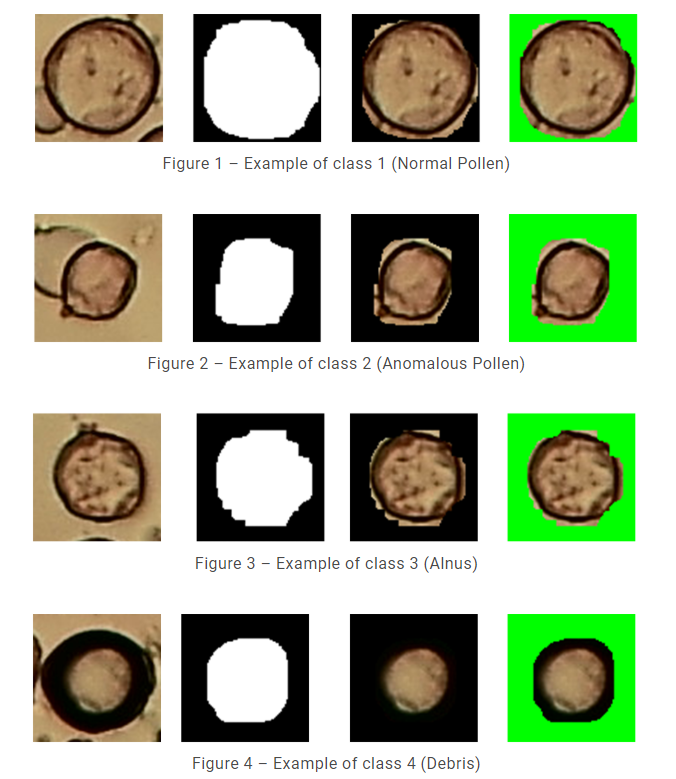
\includegraphics[width = 5in]{../cap5_experimentos/src/polen.png}
    \caption{Imagen extraída de la página oficial del Pollen Challenge \cite{polen}}
\end{figure}
% Métricas
\section{Métricas para clasificación Binaria}
% Accuracy
Analizaremos primero el caso de las métricas en un problema de clasificación binario. Es decir, dada una clase $\mathcal C$, es posible que un dato $y$ pertenezca o no pertenezca a $\mathcal{C}$.

Es importante describir primero las métricas en este tipo de problemas, debido a que cuando nos adentremos a la clasificación multiclase, estas métricas nos serán de utilidad.
\subsection{Matriz de confusión}
Considérese un problema de clasificación binarioEn el mejor de los casos, nuestro modelo podría predecir perfectamente qué datos pertenecen a nuestra clase y cuáles no lo hacen. Sin embargo, siendo que es un modelo estadístico, nuestro modelo no siempre acertará, y usando nuestros datos etiquetados podemos detectar en dónde ha habido una \textsl{confusión}. El modelo puede confundirse de dos maneras: La primera es afirmando que $y\in \mathcal C$ cuando no es el caso, y la segunda es clasificar  $y\notin \mathcal C$, cuando en realidad $y$ sí pertenecía a la clase. Por tanto, existen 4 posibilidades:

\begin{enumerate}
    \item \textbf{Verdaderos positivos}: Aquellos datos que sí pertenecen a la clase, y fueron clasificados dentro de la clase. A la cantidad de verdaderos positivos se le denota $T_P$ por sus siglas en inglés.
    \item \textbf{Falsos positivos}: Aquellos datos que sí pertenecen a la clase, y fueron clasificados fuera de la clase. A la cantidad de falsos positivos se le denota $F_P$ por sus siglas en inglés.
    \item \textbf{Verdaderos negativos}: Aquellos datos que no pertenecen a la clase, y fueron clasificados fuera de la clase. A la cantidad de verdaderos negativos se le denota $T_N$ por sus siglas en inglés.
    \item \textbf{Falsos negativos}: Aquellos datos que no pertenecen a la clase, y fueron clasificados dentro de la clase. A la cantidad de falsos negativos se le denota $F_N$ por sus siglas en inglés.
\end{enumerate}
Es posible agrupar toda esta información en una matriz conocida como \textsl{matriz de confusión}. 
\begin{definition}
    \label{pos_neg}
    Considérese el problema de clasificación (\ref{clasification}) con $m = 2$. Sea $f: \mathbb R^n \to C$ nuestro modelo. Definimos los siguientes valores:
    \begin{align*}
        T_P = |\{y_i : c_i &= (1,0)^T \text{ y } f(y_i) = (1,0)^T\}| \\
        F_P = |\{y_i : c_i &= (0,1)^T \text{ y } f(y_i) = (1,0)^T\}| \\
        T_N = |\{y_i : c_i &= (0,1)^T \text{ y } f(y_i) = (0,1)^T\}| \\
        F_N = |\{y_i : c_i &= (1,0)^T \text{ y } f(y_i) = (0,1)^T\}|.
    \end{align*} 
    La matriz de confusión se define como 
    \begin{equation}
        D = \left[\begin{matrix}
            T_P & F_P \\
            F_N & T_N
        \end{matrix}\right].
    \end{equation}
\end{definition}
\begin{figure}[H]
    \centering
    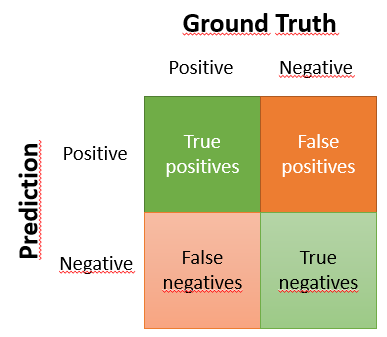
\includegraphics{../cap5_experimentos/src/matriz_confusion_binaria.png}
    \caption{\textcolor{red}{Conseguir imagen propia}}
\end{figure}
%------------- Accuracy
\subsection{Exactitud}
La exactitud se define como la razón de las predicciones acertadas y las predicciones totales. En el aprendizaje automático suele ser la métrica principal. Sin embargo, no es el único factor  a tomar en cuenta.
\begin{definition}[exactitud]
    Considérese los valores $T_P, F_P, T_N, F_N$ de la definición (\ref{pos_neg}). La exactitud $A$ se define como 
    \begin{equation}
        A = \frac{T_P + T_N}{T_P + F_P + T_N + F_N}
    \end{equation}
\end{definition}
%------------- Precisión
\subsection{Precisión}
\begin{definition}[Precisión]
    Considérese los valores $T_P, F_P, T_N, F_N$ de la definición (\ref{pos_neg}). La precisión $P$ se define como 
    \begin{equation}
        P = \frac{T_P}{T_P + F_P}
    \end{equation}
\end{definition}
%------------- Sensibilidad
\subsection{Sensibilidad}
\begin{definition}[Sensibilidad]
    Considérese los valores $T_P, F_P, T_N, F_N$ de la definición (\ref{pos_neg}). La sensibilidad $R$ se define como 
    \begin{equation}
        R = \frac{T_P}{T_P + F_N}
    \end{equation}
\end{definition}
%------------- F1-score
\subsection{\textcolor{red}{F1-score}}
\begin{definition}[\textcolor{red}{F1-score}]
    Considérese los valores $T_P, F_P, T_N, F_N$ de la definición (\ref{pos_neg}). La \textcolor{red}{F1-score} $F_1$ se define como 
    \begin{equation}
        F_1  = \frac{2}{\frac{1}{R} + \frac{1}{P}} = \frac{2RP}{R + P} = \frac{T_P}{T_P + \frac{1}{2}(F_P + F_N)}
    \end{equation}
\end{definition}
\begin{figure}[H]
    \centering
    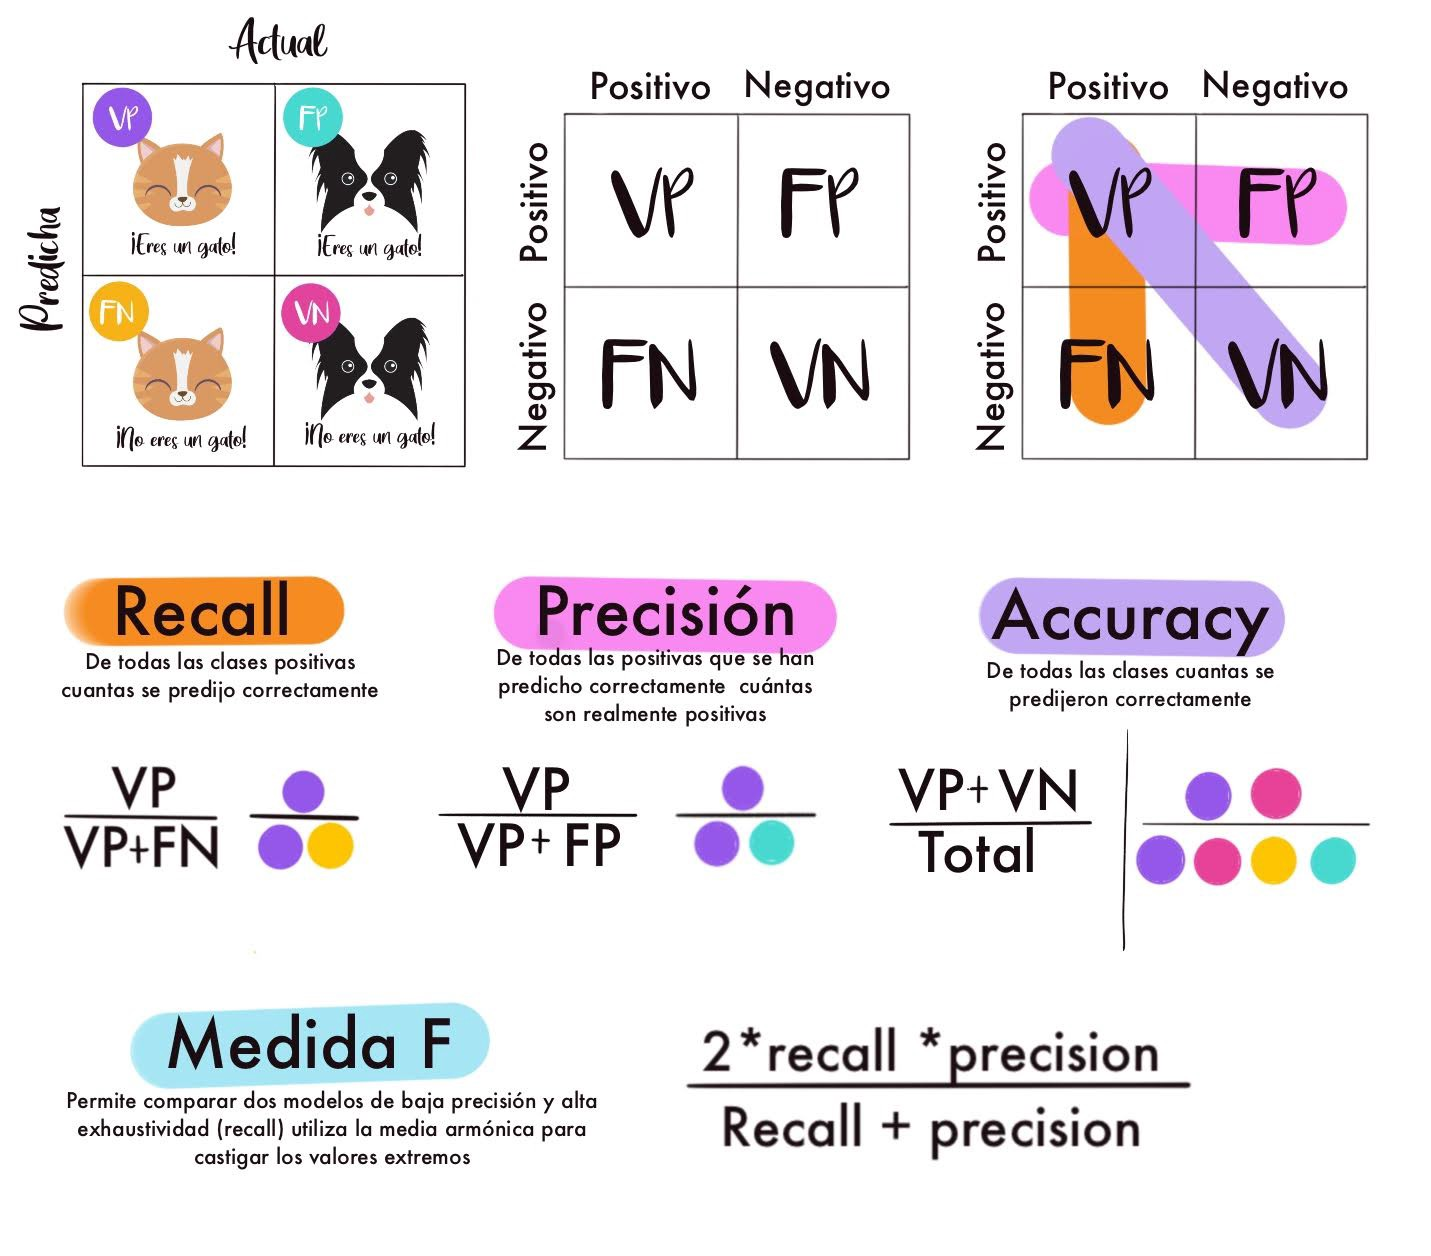
\includegraphics[width=4in]{../cap5_experimentos/src/metricas.jpeg}
\end{figure}
\section{Métricas para clasificación multiclase}
En cuanto a la problema de clasificación con múltiples clases, no podemos hacer uso directo de las fórmulas anteriores. Sin embargo, es posible conseguir una matriz de confusión. En este caso, un eje determina la verdadera etiqueta, y el otro eje determina la predicción de nuestro modelo.

\begin{figure}[H]
    \centering
    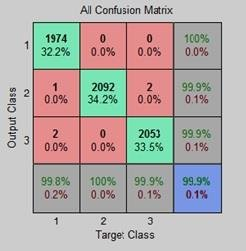
\includegraphics{../cap5_experimentos/src/confision_multiclase.png}
    \caption{\textcolor{red}{Conseguir imagen propia}}
\end{figure}
 %------------- Notas del capítulo
 \section{Notas del capítulo}
 \begin{enumerate}
     \item Añadir el libro de Suresh P. Sethi. Optimal Control Theory a las referencias.
     \item Podría añadir en la accuracy el famoso ejemplo de la predicción de cancer. donde nuestro modelo es $f(x) = 0$.
     \item Falta agregar una pequeña introducción en cada métrica de la clasificación binaria
     \item los datos de las diapositivass en la parte experimental
     \item En la referencia del pollen Challenge no aparece el URL
 \end{enumerate}
